\documentclass[10pt]{article}
\usepackage[a4paper,landscape,margin=17mm,headheight=15pt]{geometry}
\usepackage[T1]{fontenc}
\usepackage{lmodern}
\usepackage{microtype}
\usepackage{graphicx}
\usepackage{booktabs}
\usepackage{longtable}
\usepackage{array}
\usepackage{tabularx}
\usepackage{xcolor}
\usepackage{fancyhdr}
\usepackage{hyperref}
\usepackage{enumitem}

\definecolor{Ink}{HTML}{172334}
\definecolor{Accent}{HTML}{225C8F}
\definecolor{Muted}{HTML}{526172}
\definecolor{Pale}{HTML}{EAF1F7}
\hypersetup{colorlinks=true,linkcolor=Accent,urlcolor=Accent}
\setlength{\parindent}{0pt}
\setlength{\parskip}{4pt}
\setlength{\tabcolsep}{5pt}
\renewcommand{\arraystretch}{1.13}
\setlist[itemize]{topsep=2pt,itemsep=2pt,leftmargin=17pt}
\pagestyle{fancy}
\fancyhf{}
\fancyhead[L]{\small\color{Muted}HighamBench / NumStability}
\fancyhead[R]{\small\color{Muted}Accepted-proof library usage analysis}
\fancyfoot[R]{\small\thepage}
\renewcommand{\headrulewidth}{0.3pt}
\newcommand{\gain}[1]{\textbf{#1}}
\newcommand{\sourcepath}[1]{\nolinkurl{#1}}
\newcommand{\twoplot}[2]{%
  \begin{minipage}[t]{0.48\linewidth}\centering
    \includegraphics[width=\linewidth]{charts/#1.png}\\[-2pt]
    {\footnotesize\color{Muted}#2}
  \end{minipage}}

\begin{document}

\begin{center}
  {\LARGE\bfseries\color{Ink}Observed NumStability Reuse in HighamBench}\par
  \vspace{2pt}
  {\large Accepted Lean proofs across T1, T2 and T3}\par
  \vspace{4pt}
  {\small 38 tasks / 114 N--L pairs / 228 validated answers \qquad 29 September 2026}
\end{center}

\colorbox{Pale}{\parbox{0.975\linewidth}{\small
This is an observational analysis of the accepted answers underlying the repository's selected-tier results report. T1 and T2 use r11; T3 uses combined r09--r10. P16-T3 is excluded because its target was documented false. No benchmark task was rerun for this analysis.}}

\section*{Executive result}

The predicted \emph{usage} gradient is visible in the saved Lean dependency audits. It is not perfect, and it does not by itself establish that more reuse causes faster or shorter proofs.

\begin{center}
\begin{tabular}{@{}lrrrrrr@{}}
\toprule
Tier & Tasks & L runs & Any audited use & Metadata-candidate hit & Substantial tier-result hit & Median distance-1 count \\
\midrule
T1 & 12 & 36 & 33/36 & 24/36 & 30/36 & 4 \\
T2 & 3 & 9 & 9/9 & 9/9 & 9/9 & 8 \\
T3 & 23 & 69 & 9/69 & 4/69 & 0/69 & 0 \\
\bottomrule
\end{tabular}
\end{center}

\begin{minipage}[t]{0.57\linewidth}
  \vspace{0pt}\centering
  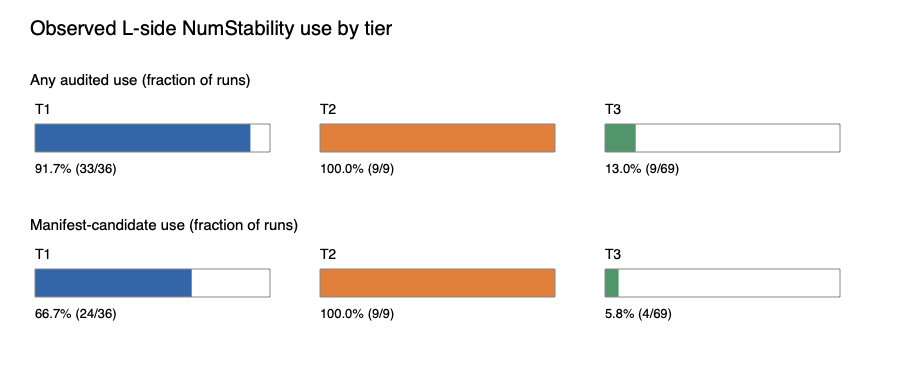
\includegraphics[width=\linewidth]{charts/tier_usage.png}
\end{minipage}
\hfill
\begin{minipage}[t]{0.40\linewidth}
  \vspace{0pt}
  {\large\bfseries Principal interpretation}\par
  \smallskip
  Across the 38 task means, the candidate-aware score has Spearman correlation $+0.62$ with time gain and $+0.53$ with physical-LOC gain. These are \emph{across-tier} associations. Within T1, the corresponding values are $-0.27$ and $-0.20$; within T3 they are $+0.03$ and $-0.33$. There is no universal within-tier monotonic gain rule.

  P15-T3 uses NumStability matrix/norm lemmas in all three repetitions, but has no corresponding aggregate result. N has zero audited NumStability use in all 114 pairs.
\end{minipage}

\clearpage
\section{Corpus and measurement design}

The analysis takes the selected paired repetitions from \sourcepath{../live-r11/completed_pairs.csv} for T1/T2 and \sourcepath{../combined-r09-r10/completed_pairs.csv} for T3. Each task contributes three accepted N/L pairs. The repository's \sourcepath{metadata/manifest.json} supplies task-listed candidate declarations and tier rationales; a separate, transparent \sourcepath{semantic_catalog.json} lists substantial T1/T2 results and documented alternatives. These last two classifications are retrospective, not independently authenticated campaign-time treatment assignments.

Every input attempt must have a passing final validation and complete hidden Lean dependency audit. The reproducer checks the accepted-proof SHA-256 against its attempt record, pair and condition identity, summary time/token/LOC against that record, and absence of NumStability dependencies in N. The 228 accepted proof and attempt paths and hashes are in \sourcepath{attempt_usage.csv}.

\subsection*{Complementary measures of use}

\begin{tabularx}{\linewidth}{@{}p{0.21\linewidth}X@{}}
\toprule
Measure & Operational meaning and limitation \\
\midrule
Import count & Number of distinct imported NumStability modules. Availability is not use. \\
Qualified source names & Distinct and repeated \texttt{NumStability.*} references outside imports, comments and strings. Can count rewrites or code outside the accepted theorem's dependency closure. \\
Qualified live names & Qualified source references that name something in the accepted target's audited closure. Approximate name matching; unqualified references can be missed. \\
Distance-1 count & NumStability declarations one edge from the target theorem in the saved Lean dependency graph. This is near/direct graph reach, not necessarily one explicit tactic application. \\
Transitive count & All NumStability declarations in the target's dependency closure, including support code. It is a footprint, not a count of intentional theorem uses. The filtered version omits several compiler-generated name patterns, but is not a complete public-API classifier. \\
Metadata-candidate hits & Intersection with the repository's task-listed \texttt{candidate\_library\_dependencies\_for\_audit}. The list is not exhaustive. \\
Substantial-result hits & Audited use of a task-relevant theorem named by a T1/T2 tier rationale or a documented alternative. T3 has no predesignated result by definition, so this is not an independent tier test. \\
\bottomrule
\end{tabularx}

\subsection*{Two ordinal scores}

The candidate-aware score is 0 for no audited dependency, 1 for audited library use without a task-listed candidate, 2 for one candidate hit, and 3 for two or more candidate hits. The substantial-result score is 0 for no audited use, 1 for use without a cataloged substantial result, 2 when such a result appears in the accepted theorem's closure, and 3 when at least two are also explicitly named in accepted source. Task scores are medians of three repetitions. Neither score measures latent library coverage or proves causal leverage.

\subsection*{Outcome measures}

Gain is $(N-L)/N\times 100\%$; positive favors L. Task gains use the arithmetic mean of N and L over three repetitions. Elapsed time ends at the authenticated accepted submission. Physical LOC counts submitted source, not imported library code. Every selected token record is incomplete, so token figures and gains are observed lower-bound comparisons only.

\clearpage
\section{Task-by-task results}

The table retains every selected task. ``Score'' is the candidate-aware median; ``Use'' and ``Cand.'' are the number of three L repetitions with any audited library dependency and at least one metadata-candidate hit, respectively. The full numerical measures and exact declaration names remain in the accompanying CSV files.

\footnotesize
\setlength{\tabcolsep}{12pt}
\renewcommand{\arraystretch}{1.0}
\begin{longtable}{@{}llrrrrrr@{}}
\caption{Observed usage and N-over-L task-mean gains. Positive gains favor L. Token gains are lower-bound comparisons.}\label{tab:tasks}\\
\toprule
Task & Tier & Score & Use & Cand. & Time gain & Token gain & LOC gain \\
\midrule
\endfirsthead
\toprule
Task & Tier & Score & Use & Cand. & Time gain & Token gain & LOC gain \\
\midrule
\endhead
P01-T1 & T1 & 2 & 2/3 & 2/3 & +52.4\% & +47.6\% & +39.2\% \\
P01-T2 & T2 & 3 & 3/3 & 3/3 & +75.3\% & +65.6\% & +60.0\% \\
P02-T1 & T1 & 2 & 3/3 & 3/3 & +16.2\% & -26.9\% & +4.7\% \\
P02-T3 & T3 & 0 & 1/3 & 0/3 & -19.9\% & -209.4\% & -10.7\% \\
P03-T3 & T3 & 0 & 0/3 & 0/3 & -14.5\% & -79.0\% & -0.5\% \\
P04-T1 & T1 & 2 & 3/3 & 3/3 & +11.2\% & -10.0\% & +13.8\% \\
P05-T3 & T3 & 0 & 0/3 & 0/3 & +9.0\% & -24.9\% & +10.1\% \\
P06-T3 & T3 & 0 & 0/3 & 0/3 & +11.6\% & +43.3\% & +1.0\% \\
P08-T3 & T3 & 0 & 0/3 & 0/3 & +33.0\% & +49.8\% & +6.7\% \\
P09-T3 & T3 & 0 & 0/3 & 0/3 & +7.9\% & +11.4\% & -9.0\% \\
P11-T3 & T3 & 0 & 0/3 & 0/3 & -7.1\% & -9.7\% & +2.5\% \\
P12-T1 & T1 & 3 & 3/3 & 3/3 & +52.8\% & -19.4\% & +49.1\% \\
P13-T3 & T3 & 0 & 0/3 & 0/3 & +29.4\% & +35.1\% & -3.2\% \\
P14-T1 & T1 & 2 & 3/3 & 3/3 & +17.7\% & +11.1\% & -7.3\% \\
P15-T1 & T1 & 2 & 3/3 & 3/3 & +75.1\% & +55.2\% & +59.2\% \\
P15-T2 & T2 & 3 & 3/3 & 3/3 & +76.6\% & +78.2\% & +62.8\% \\
P15-T3 & T3 & 3 & 3/3 & 3/3 & +10.3\% & +17.0\% & -11.0\% \\
P17-T1 & T1 & 0 & 1/3 & 0/3 & +21.0\% & -41.0\% & +17.2\% \\
P17-T3 & T3 & 0 & 0/3 & 0/3 & +4.2\% & +2.7\% & -9.7\% \\
P19-T3 & T3 & 0 & 0/3 & 0/3 & +13.6\% & +55.3\% & -3.0\% \\
P20-T3 & T3 & 0 & 1/3 & 1/3 & +14.0\% & -2.5\% & -11.8\% \\
P23-T1 & T1 & 3 & 3/3 & 3/3 & +62.5\% & +28.1\% & +41.0\% \\
P24-T3 & T3 & 0 & 0/3 & 0/3 & -22.4\% & +11.9\% & -19.9\% \\
P25-T3 & T3 & 0 & 0/3 & 0/3 & -2.6\% & +10.5\% & -9.2\% \\
P26-T1 & T1 & 2 & 3/3 & 3/3 & +71.9\% & +67.0\% & +67.7\% \\
P27-T3 & T3 & 0 & 0/3 & 0/3 & +4.6\% & -9.5\% & +5.6\% \\
P28-T1 & T1 & 1 & 3/3 & 0/3 & +77.3\% & +69.1\% & +57.0\% \\
P28-T3 & T3 & 0 & 0/3 & 0/3 & -7.9\% & +37.5\% & +10.2\% \\
P29-T1 & T1 & 1 & 3/3 & 0/3 & +76.8\% & +62.0\% & +69.3\% \\
P29-T2 & T2 & 3 & 3/3 & 3/3 & +61.8\% & +61.0\% & +58.5\% \\
P32-T3 & T3 & 0 & 0/3 & 0/3 & -7.6\% & -50.4\% & -2.4\% \\
P33-T1 & T1 & 1 & 3/3 & 1/3 & +70.8\% & +40.6\% & +58.4\% \\
P34-T3 & T3 & 0 & 0/3 & 0/3 & +23.8\% & +15.5\% & +5.1\% \\
P35-T3 & T3 & 1 & 2/3 & 0/3 & -8.1\% & -1.1\% & -3.6\% \\
P36-T3 & T3 & 0 & 0/3 & 0/3 & -1.4\% & -20.1\% & -21.4\% \\
P37-T3 & T3 & 0 & 0/3 & 0/3 & +2.4\% & +56.4\% & -8.4\% \\
P39-T3 & T3 & 0 & 0/3 & 0/3 & +25.2\% & +29.9\% & +5.3\% \\
P40-T3 & T3 & 1 & 2/3 & 0/3 & +13.9\% & +1.4\% & -11.9\% \\
\bottomrule
\end{longtable}
\normalsize
\setlength{\tabcolsep}{5pt}
\renewcommand{\arraystretch}{1.13}

\clearpage
\section{Use versus proof size and time}

Each point represents the arithmetic mean of three N/L repetitions for a task; color denotes tier. The x-axis is the median candidate-aware score. Every selected task is shown, including losses and mixed-use cases.

\begin{center}
\twoplot{score_vs_loc}{Physical-LOC gain versus candidate-aware use}
\hfill
\twoplot{score_vs_time}{Elapsed-time gain versus candidate-aware use}
\end{center}

\begin{center}
\twoplot{score_vs_tokens}{Observed-token gain versus candidate-aware use}
\hfill
\begin{minipage}[t]{0.48\linewidth}
\small
\textbf{Task means grouped by median candidate score}\\[3pt]
\begin{tabular}{@{}rrrrrr@{}}
\toprule
Score & Tasks & Mean time & Mean LOC & L faster & L shorter \\
\midrule
0 & 21 & +5.5\% & -2.2\% & 13/21 & 9/21 \\
1 & 5 & +46.1\% & +33.8\% & 4/5 & 3/5 \\
2 & 6 & +40.7\% & +29.6\% & 6/6 & 5/6 \\
3 & 6 & +56.5\% & +43.4\% & 6/6 & 5/6 \\
\bottomrule
\end{tabular}

\vspace{6pt}
The grouped mean is descriptive: score, tier and mathematical difficulty are entangled. Score 1 is not weaker evidence than score 0 for every outcome, and score 3 includes the P15-T3 exception. Token counts are incomplete lower bounds.
\end{minipage}
\end{center}

\clearpage
\section{Alternative semantic score and stratified associations}

The substantial-result score checks the T1/T2 tier-rationale theorems and documented alternatives rather than simply counting all listed candidates. It is useful for interpretation but partly constructed from the tier design; it cannot independently validate that design.

\begin{center}
\twoplot{substantial_vs_loc}{Physical-LOC gain versus substantial-result score}
\hfill
\twoplot{substantial_vs_time}{Elapsed-time gain versus substantial-result score}
\end{center}

\small
\begin{center}
\begin{tabular}{@{}lrrrrrrrr@{}}
\toprule
Group & Tasks & Cand./time & Cand./LOC & Cand./tokens & Subst./time & Subst./LOC & Distance-1/time & Distance-1/LOC \\
\midrule
All & 38 & +0.62 & +0.53 & +0.36 & +0.69 & +0.63 & +0.63 & +0.59 \\
T1 & 12 & -0.27 & -0.20 & -0.17 & +0.09 & +0.03 & -0.13 & -0.02 \\
T2 & 3 & n/a & n/a & n/a & n/a & n/a & -0.50 & -0.50 \\
T3 & 23 & +0.03 & -0.33 & -0.01 & +0.02 & -0.33 & -0.03 & -0.24 \\
\bottomrule
\end{tabular}
\end{center}
\normalsize

All values are task-level Spearman rank correlations with average ranks for ties. ``n/a'' means the score does not vary within the three T2 tasks. No $p$-value or causal claim is made. The complete matrix of eleven predictors by three outcomes, overall and within tier, is in \sourcepath{associations.csv}.

\clearpage
\section{Mixed-use repetitions and diagnostic cases}

Six tasks contain both a library-using and a non-using L repetition. Comparing paired N/L gains within the same task controls task identity, but not random variation or the agent's decision to use the library; this is exploratory.

\begin{center}
\begin{tabular}{@{}llrrrr@{}}
\toprule
Task & Tier & Using runs & Non-using runs & Mean time gain: use / no use & Mean LOC gain: use / no use \\
\midrule
P01-T1 & T1 & 2 & 1 & +76.8\% / -12.4\% & +64.2\% / -24.8\% \\
P02-T3 & T3 & 1 & 2 & -12.4\% / -25.3\% & -22.3\% / -5.2\% \\
P17-T1 & T1 & 1 & 2 & +24.6\% / +18.7\% & +31.4\% / +8.3\% \\
P20-T3 & T3 & 1 & 2 & +16.2\% / +13.1\% & -0.4\% / -18.2\% \\
P35-T3 & T3 & 2 & 1 & -10.5\% / -4.3\% & -8.8\% / +6.1\% \\
P40-T3 & T3 & 2 & 1 & +13.2\% / +12.8\% & -23.4\% / +5.9\% \\
\bottomrule
\end{tabular}
\end{center}

\begin{itemize}
\item \textbf{P01-T1:} one run has no audited library use; the two using runs show much larger time and LOC gains. This is suggestive, not conclusive with three repetitions.
\item \textbf{P01-T2:} all three L proofs use the three substantial summation bounds. Its mean time and LOC gains are +75.3\% and +60.0\%.
\item \textbf{P15-T3:} all three L proofs use nearby matrix/norm lemmas, yet L's mean submitted LOC is 11.0\% greater. This prevents a blanket claim that any library use shortens code.
\item \textbf{P17-T1:} only one of three L proofs has an audited library dependency; none reaches the substantial tier-rationale theorem. The task-level candidate score is 0 despite one using repetition.
\end{itemize}

The complete per-repetition comparisons, including observed tokens, are in \sourcepath{mixed_task_usage.csv}. The name-level declaration inventory is \sourcepath{declaration_usage.csv}; it records the frequency of all 325 distinct audited library declarations and their distance-1 incidence.

\clearpage
\section{Provenance, limitations and reproduction}

The primary evidence is each saved \texttt{attempt.json} hidden Lean dependency audit, not a text match. The analysis also stores raw source counts for comparison. \sourcepath{attempt_usage.csv} gives every accepted proof and attempt-record path and SHA-256. \sourcepath{pair_usage.csv} joins N and L. \sourcepath{task_usage.csv} supplies the plotted task means. \sourcepath{input_hashes.json} fixes the manifest, semantic catalog and two summary CSV inputs.

Four of the 228 attempt records contain a final on-disk candidate hash different from the accepted-proof hash. The analysis consistently uses the validated \texttt{accepted\_proof.lean} that was used for scoring; the distinct later terminal files are not archived here. All 114 N/L selected pairs have both accepted proofs, pass flags and complete saved library audits.

\subsection*{Limits on interpretation}

\begin{itemize}
\item Task tiers were designed using anticipated library support, and this is a selected corpus. The semantic map is based on tier rationales and documented alternatives, so cross-tier association is partly built into the classification.
\item T2 contains only three tasks. Three repetitions of one task do not constitute three independent papers.
\item A transitive dependency count can be inflated by a single invoked theorem's implementation. A lexical count can miss unqualified names or include code outside the accepted theorem's dependency closure.
\item Library material may be available yet unused. The current repository does not contain complete conversations or every draft, so search effort and abandoned approaches cannot be reconstructed from this dataset.
\item Every selected token record is incomplete. Observed-token differences must not be described as exact token savings.
\item The saved audit covers the accepted target theorem as a whole. A separate Lean instrument would be needed to partition every dependency exactly into statement versus proof-term use.
\end{itemize}

\subsection*{Reproduce this analysis}

From the repository root, run:
\begin{quote}\ttfamily
python3 paper\_bencmark/highambench/reports/library-usage-analysis/analyze.py
\end{quote}
The script uses only Python's standard library and regenerates the CSV, SVG and Markdown outputs beside itself. For this PDF, PNG renderings of the SVG plots are stored in \sourcepath{charts/}; compile \sourcepath{report.tex} with \texttt{latexmk -pdf}. The accompanying \sourcepath{test_analyze.py} checks the lexical scanner and score boundaries. No measurement record is changed by report generation.

\smallskip
\textbf{Repository paths.}
\begin{itemize}
\item Source summaries: \sourcepath{../live-r11/completed_pairs.csv} and \sourcepath{../combined-r09-r10/completed_pairs.csv}.
\item Task metadata: \sourcepath{../../metadata/manifest.json}.
\item Prior rationale audit: \sourcepath{../combined-r09-r10/library_dependency_audit.md}.
\item Output tables, plots and source hashes: this \sourcepath{library-usage-analysis/} directory.
\end{itemize}

\end{document}
